\begin{tikzpicture}[font=\bf\sffamily\fontsize{9}{9}\selectfont]

  
\node[] (A) at (0,0) {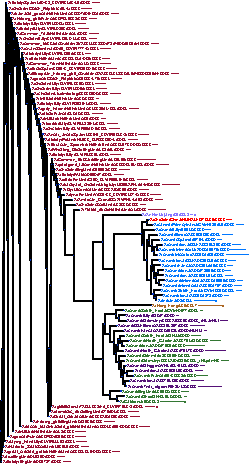
\includegraphics[width=.9\textwidth]{Figures/riskyphylo6.25_collapsed_20}};

\draw[line width=6pt] ([yshift=.5in,xshift=1.28in]A.south) node (DA) [left,below]{6.0} -- ++(.7in,0) node (DB) [right,below] {6.7};
\node[anchor=south] (L1)  at ([yshift=.1in]$(DA.north)!.5!(DB.north)$) {estimated IRAT emergence score};

\coordinate (C1) at ([xshift=-.125in,yshift=1in]L1.north) ;

\node[align=center,fill=Red4!80!black,text=white,,text width=.35in,anchor=north,xshift=-0.05in,yshift=-.30in,label={[font=\bf\sffamily\fontsize{9}{9}\selectfont,
  xshift=.2in,yshift=.1in,text=gray]90:subtypes of risky strains}] (X1) at (C1.south) {H1N1};
\node[align=center,text=white,fill=Blue1!80,text width=.35in,anchor=north,xshift=0in,yshift=-.051in] (X2) at (X1.south) {H3N2};
\node[align=center,text=white,fill=DarkOrange2,text width=.35in,anchor=west,xshift=0.02in,yshift=0in] (X1) at (X1.east) {H9N2};
\node[text=white,align=center,fill=Green4,text width=.35in,anchor=north,xshift=0in,yshift=-.051in] (X1) at (X1.south) {H7N9};

\def\FCOLX{Red1}


\node[shape=isosceles triangle,fill=\FCOLX,rotate=90 ] (h1n1strain) at ([xshift=-.95in,yshift=1.850in]L1.north) {};

\node[anchor=west] at ([xshift=.1in,yshift=-.1in]h1n1strain.east) {
\includegraphics[width=.5in]{Figures/animalicons/pig}};

\node[shape=isosceles triangle,fill=\FCOLX,rotate=-90 ] (h7n9strain) at ([xshift=.850in,yshift=4.65in]L1.north) {};
\node[anchor=west] at ([xshift=-.2in,yshift=0.45in]h7n9strain.east) {
\includegraphics[width=.6in]{Figures/animalicons/camel}};

\node[shape=isosceles triangle,fill=\FCOLX,rotate=-90 ] (h3n2strain) at ([xshift=1.22in,yshift=4.1in]L1.north) {};
\node[anchor=west] at ([xshift=-.2in,yshift=0.35in]h3n2strain.east) {
\includegraphics[width=.4in]{Figures/animalicons/pig}};

\node[shape=isosceles triangle,fill=\FCOLX,rotate=-90 ] (h9n2strain) at ([xshift=.3in,yshift=4.8in]L1.north) {};
\node[anchor=west] (mink) at ([xshift=-.265in,yshift=0.35in]h9n2strain.east) {
\includegraphics[width=.6in]{Figures/animalicons/mink}};

\node[anchor=west,opacity=.5] (cc) at ([xshift=-3in,yshift=-1in]h9n2strain.east) {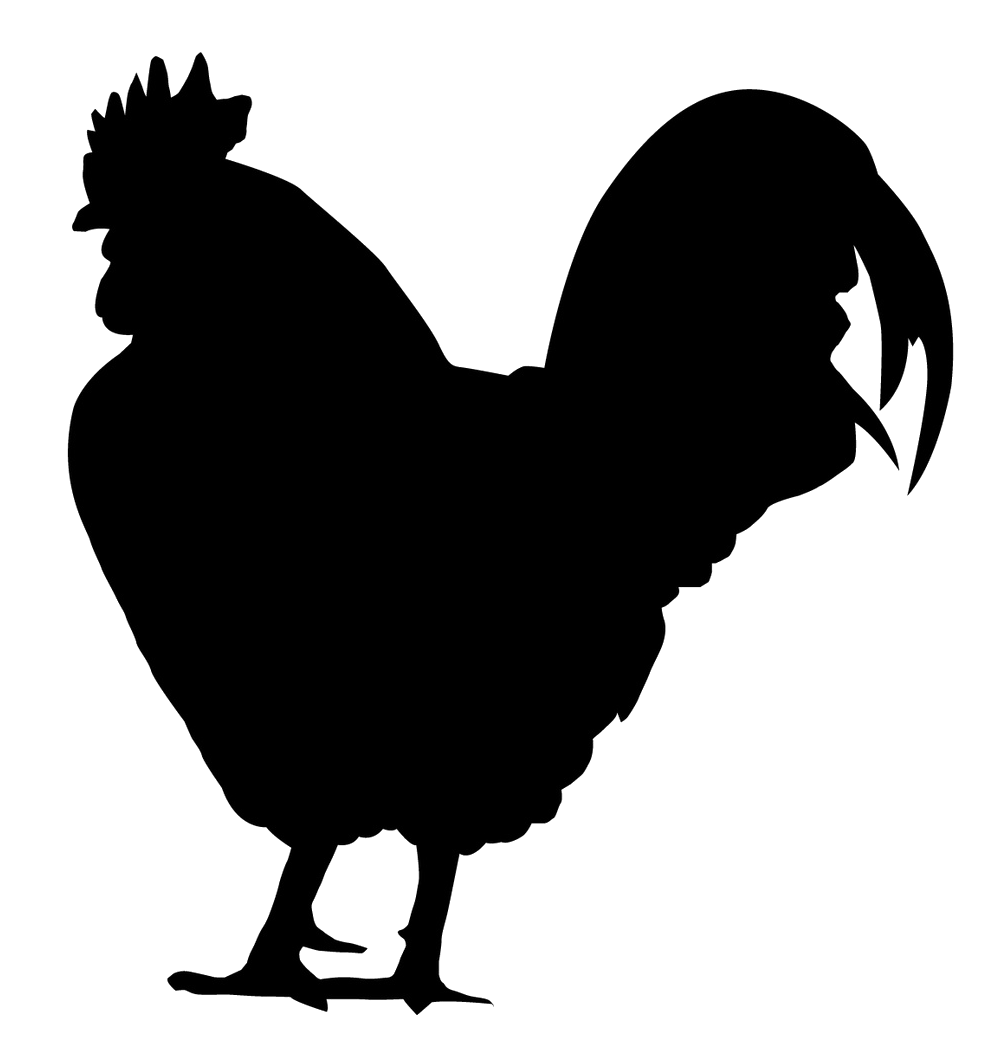
\includegraphics[width=.5in]{Figures/animalicons/chicken}};
\node[anchor=west,opacity=.5] (dd) at ([xshift=-2.5in,yshift=-1.45in]h9n2strain.east) {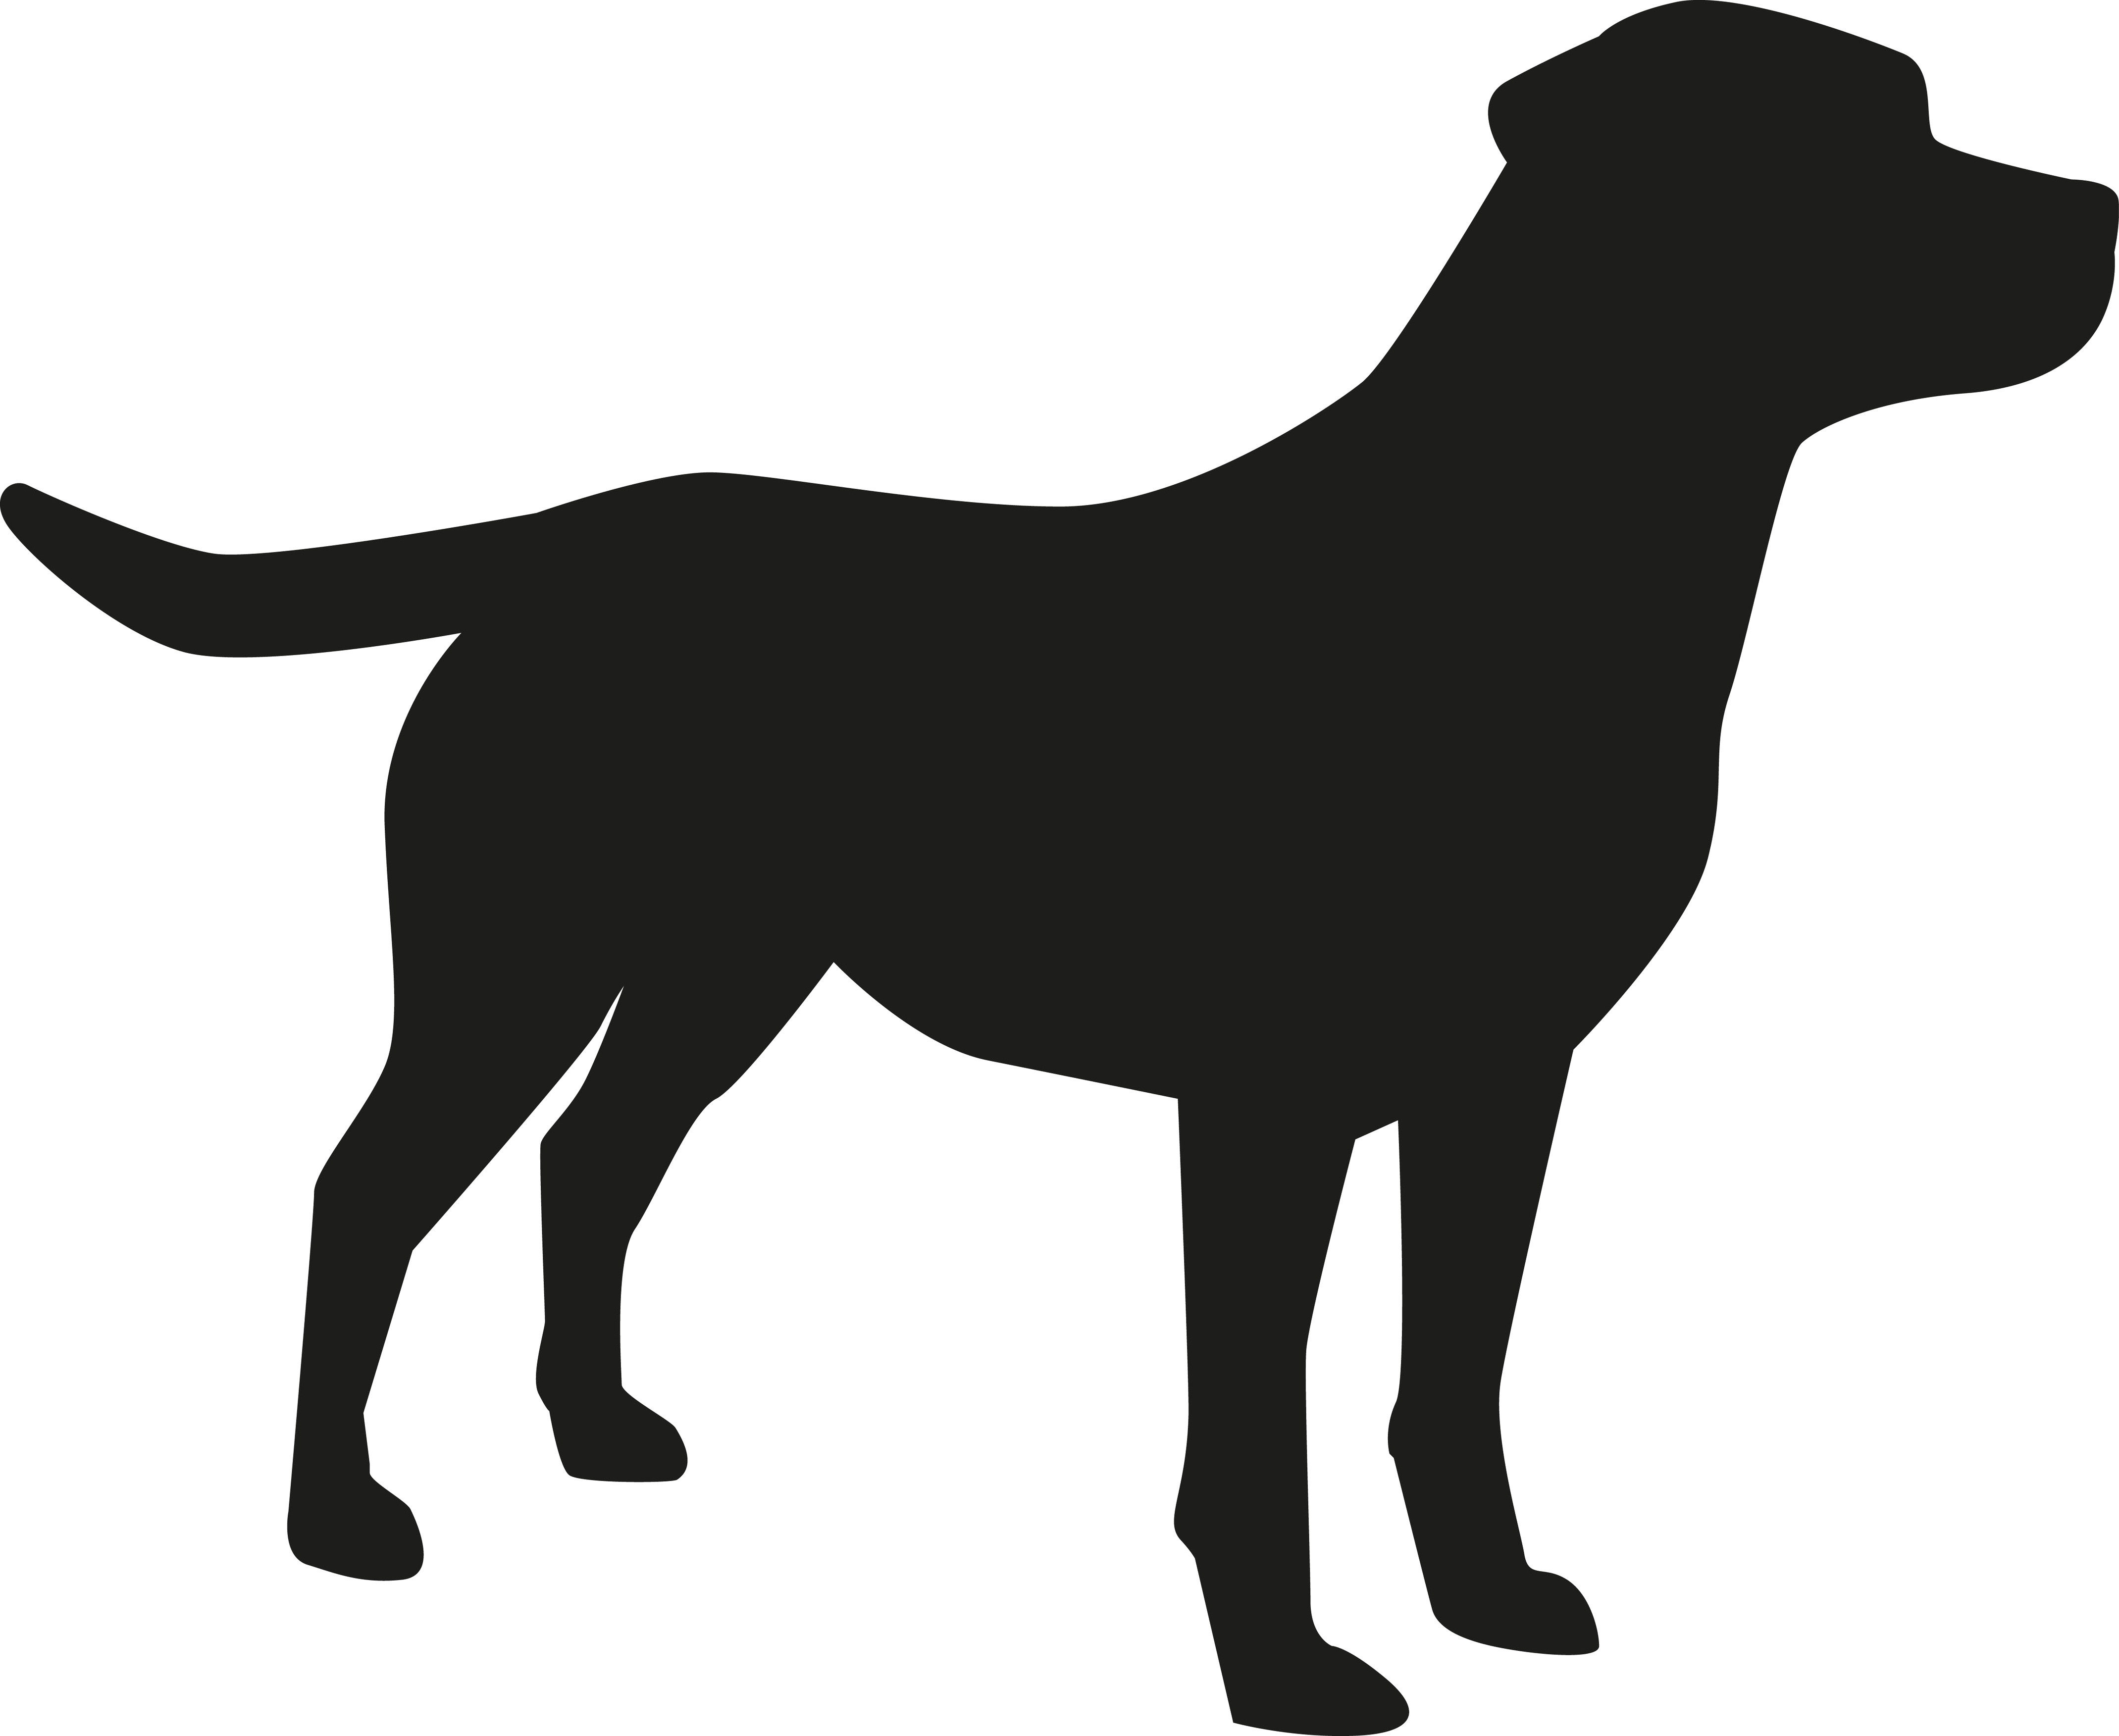
\includegraphics[width=.6in]{Figures/animalicons/dog}};
\node[anchor=west,opacity=.5] (dc) at ([xshift=-2in,yshift=-1.85in]h9n2strain.east) {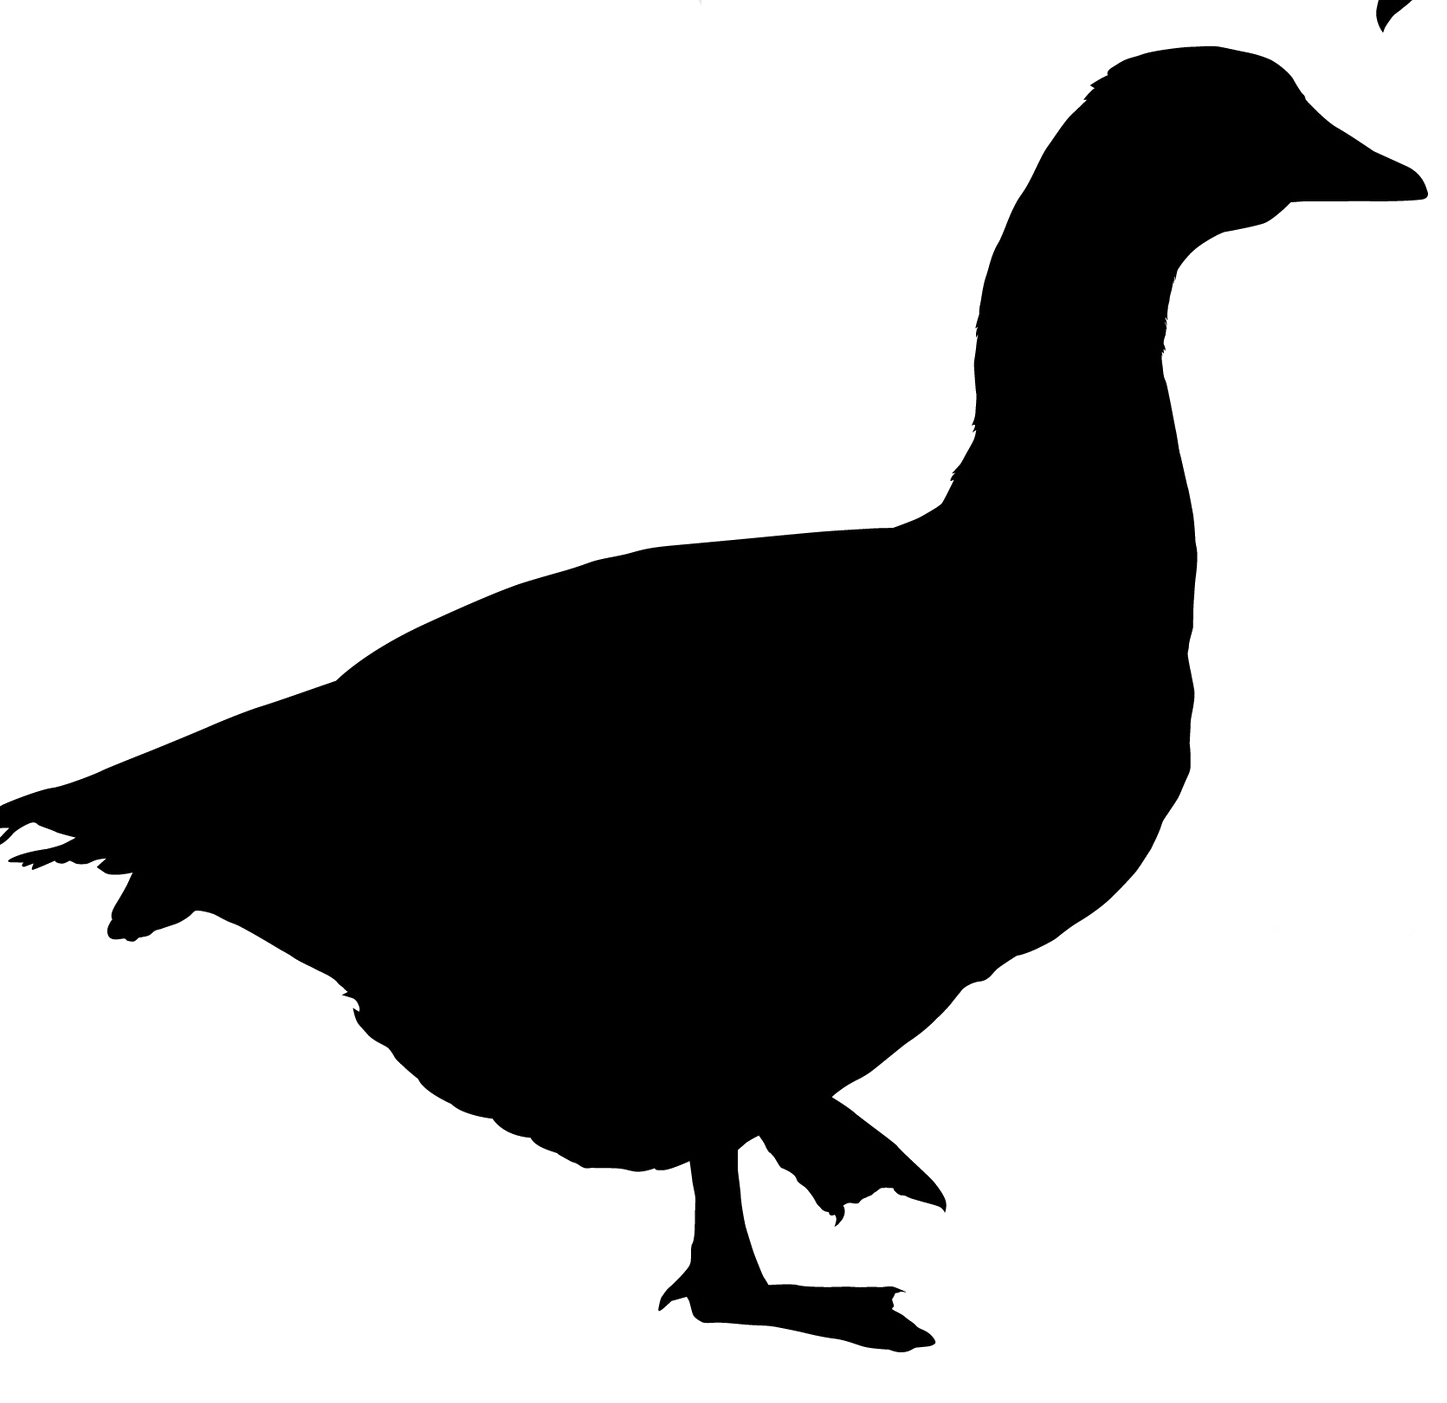
\includegraphics[width=.5in]{Figures/animalicons/duck2}};

\node[anchor=south,opacity=.4] (pig2) at ([xshift=-2.2in,yshift=-5.5in]mink.north) {
\includegraphics[width=.8in]{Figures/animalicons/pig}};

\node[anchor=south,opacity=.4] (pig3) at ([xshift=-1in,yshift=1in]mink.north) {
\includegraphics[width=.8in]{Figures/animalicons/pig}};


\draw [ultra thick,dashed,opacity=.3] (cc) -- ++(1.1in,1in);
\draw [ultra thick,dashed,opacity=.3] (dd) -- ++(.96in,1in);
\draw [ultra thick,dashed,opacity=.3] (dc) -- ++(.55in,1.3in);
% \draw [ultra thick,dashed,opacity=.3] (pig3) -- ++(-.8in,-1.5in);
% \draw [ultra thick,dashed,opacity=.3] (pig3) -- ++(-1.6in,0in);
% \draw [ultra thick,dashed,opacity=.3] (pig3) -- ++(-1.6in,1.5in);
% \draw [ultra thick,dashed,opacity=.3] (pig2) -- ++(-.8in,-1.5in);
% \draw [ultra thick,dashed,opacity=.3] (pig2) -- ++(-1.6in,0in);
% \draw [ultra thick,dashed,opacity=.3] (pig2) -- ++(-1.6in,1.5in);

% \coordinate (CC) at ([xshift=1.5in]h1n1strain);
% \draw[opacity=.15] (h1n1strain) -- (CC);
% \draw[opacity=.15] (h3n2strain) -- (CC);
% \draw[opacity=.15] (h7n9strain) -- (CC);
% \draw[opacity=.15] (h9n2strain) -- (CC);

\end{tikzpicture}